\section{Introduction} \label{sec:intro}

% \XX{do you cite olson??} \sXX{now cited}

% applications of socially aware navigation (robots)
Recent advances in sensing and computing technologies have spurred greater interest in various applications of autonomous ground vehicles. In particular, researchers have explored using robots to provide personal mobility services and luggage carrying support in complex, pedestrian-rich environments (e.g., airports and shopping malls)~\cite{bai_intention-aware_2015}. These tasks often require the robots to be capable of navigating efficiently and safely in close proximity of people, which is challenging because pedestrians tend to follow subtle social norms that are difficult to quantify, and pedestrians' intents (i.e., goals) are usually not known~\cite{kretzschmar_socially_2016}.

% prediction + static motion planner -> freezing robot problem
A common approach treats pedestrians as dynamic obstacles with simple kinematics, and employs specific reactive rules for avoiding collision~\cite{fox_dynamic_1997,van_den_berg_reciprocal_2008,phillips_sipp:_2011,berg_reciprocal_2011}. Since these methods do not capture human behaviors, they sometimes generate unsafe/unnatural movements, particularly when the robot operates near human walking speed~\cite{kretzschmar_socially_2016}. To address this issue, more sophisticated motion models have been proposed, which would reason about the nearby pedestrians' hidden intents to generate a set of predicted paths~\cite{kim_brvo:_2015,unhelkar_human-robot_2015}. Subsequently, classical path planning algorithms would be employed to generate a collision-free path for the robot. Yet, separating the navigation problem into disjoint prediction and planning steps can lead to the \emph{freezing robot problem}, in which the robot fails to find any feasible action because the predicted paths could mark a large portion of the space untraversable~\cite{trautman_robot_2015}.
%\mXX{they have a newer journal paper extending the freezing robot problem, which might worth citing, \url{http://journals.sagepub.com/doi/pdf/10.1177/0278364914557874.}} \sXX{added reference to this new work}
A key to resolving this problem is to account for cooperation, that is, to model/anticipate the impact of the robot's motion on the nearby pedestrians. 

\begin{figure}[t]
	\centering
%	\includegraphics [trim=0 0 0 0, clip, angle=0, width=0.8\columnwidth, keepaspectratio]{figures/stata_nav}
	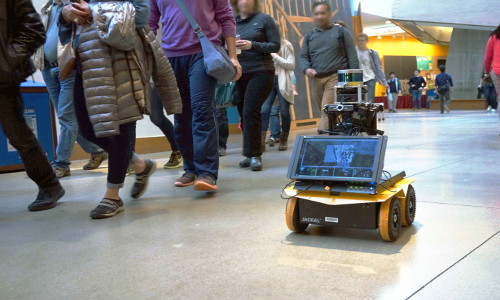
\includegraphics [trim=0 0 0 0, clip, angle=0, width=0.8\columnwidth,
	keepaspectratio]{figures/rover_d}
	\caption{A robotic vehicle navigating autonomously in a pedestrian-rich environment. Accounting for social interactions is important for operating such vehicles safely and smoothly. %\sXX{will take a better pic}
	} 
	\label{fig:rover} 
	%\vskip -0.1in
\end{figure}

%\XX{\color{red} many weak sentences in the following - make it sharper and more clear} \sXX{reworded}
% cooperative methods (behabivor approach - BRVO, social forces)
%Existing work on cooperative, socially compliant navigation can be broadly classified into two categories, namely \textit{model-based} and \textit{learning-based}. Model-based approaches are typically extensions of multiagent collision avoidance algorithms, with additional tuned parameters to account for human--human and human--robot interactions~\cite{helbing_social_1995,ferrer_robot_2013,kim_brvo:_2015}. These methods \XX{are computationally efficient, - how do you know? seems like an odd statement - it might be how they re designed} but \XX{might not capture - \color{red} not a great statement at all} the complexity of human behaviors. In particular, \XX{the parameters - we don't know what you are talking about here} can vary 
%\XX{do you mean that the parameter settings needed can be highly dependent on the scenario and the particular pedestrians??}
%significantly among pedestrians and these methods can lead to generating oscillatory trajectories~\cite{kretzschmar_socially_2016,chen_decentralized_2017}.

Existing work on cooperative, socially compliant navigation can be broadly classified into two categories, namely \textit{model-based} and \textit{learning-based}. Model-based approaches are typically extensions of multiagent collision avoidance algorithms, with additional parameters introduced to account for social interactions~\cite{helbing_social_1995,ferrer_robot_2013,ferrer_behavior_2014,kim_brvo:_2015,mehta_autonomous_2016}. For instance, to distinguish between human--human and human--robot interactions, the extended social forces model~\cite{ferrer_behavior_2014,ferrer_robot_2013} augments the potential field algorithm with additional terms that specify the repulsive forces (e.g., strength and range) governing each type of interaction. Model-based methods are designed to be computationally efficient as they often correspond to intuitive geometric relations; yet, it is unclear whether humans do follow such precise geometric rules. In particular, the force parameters often need to be tuned individually, and can vary significantly for different pedestrians~\cite{ferrer_behavior_2014}. Also, it has been observed that model-based methods can lead to oscillatory paths~\cite{chen_decentralized_2017,kretzschmar_socially_2016}. %Recent work has proposed switching between a few model-based approaches~\cite{mehta_autonomous_2016}, which can lead to having more parameters to tune. 

% cooperative methods (learning based approach - inverse RL, max entropy)
In comparison, learning-based approaches aim to develop a policy that emulates human behaviors by matching feature statistics, such as the minimum separation distance to pedestrians. In particular, Inverse Reinforcement Learning (IRL)~\cite{abbeel_apprenticeship_2004} has been applied to learn a cost function from human demonstration (teleoperation)~\cite{kim_socially_2015}, and a probability distribution over the set of joint trajectories with nearby pedestrians~\cite{kuderer_feature-based_2012,kretzschmar_socially_2016}. Compared with model-based approaches, learning-based methods have been shown to produce paths that more closely resemble human behaviors, but often at a much higher computational cost. This is because computing/matching trajectory features often requires anticipating the joint paths of all nearby pedestrians~\cite{kretzschmar_socially_2016}, and might depend on some  unobservable information (e.g., pedestrians' goals). 
%5
More importantly, since human behaviors are inherently stochastic, 
%\XX{paths - is the issue here paths or behaviors? my path might change even though my behavior doesn't} \sXX{the feature statistics can differ due to stochasticity in people's behavior, so feature matching won't work/generalize so well. } 
the feature statistics calculated on pedestrians' paths can vary significantly from person to person, and even run to run for the same scenario~\cite{kim_socially_2015,kretzschmar_socially_2016}. This raises concerns over whether such feature-matching methods are generalizable to different environments~\cite{mehta_autonomous_2016}.

% main challenge
%\mXX{The transition seems not smooth. previous two paragraphs talked two categoies of methods and their issues. Might want to remind reader that the proposed method is also learning based or something else and those issues in the previous methods} \sXX{good point, need to address this comment}
%In short, due to the stochasticity in people's behaviors, socially compliant navigation remains difficult to quantify despite being instinctive to humans. \XX{thought flow from last sentence to here doesn't make sense} Yet, it has been widely observed that human navigation (or teleoperation) is time-efficient and generally respects a set of simple social norms (i.e., ``passing on the right'')~\cite{kim_socially_2015,kretzschmar_socially_2016,knepper_pedestrian-inspired_2012}. We note that while it is challenging to directly specify the details of \emph{what to do} (precise mechanisms of human navigation), it is straightforward to specify \emph{what not to do} (violations of social norms).

In short, existing works are mostly focused on modeling and replicating the detailed mechanisms of social compliance, which remains difficult to quantify due to the stochasticity in people's behaviors. In comparison, humans can intuitively evaluate whether a behavior is acceptable. In particular, human navigation (or teleoperation) is time-efficient and generally respects a set of simple social norms (e.g., ``passing on the right'')~\cite{kim_socially_2015,kretzschmar_socially_2016,knepper_pedestrian-inspired_2012}. %Moreover, we note that while it is challenging to directly specify the details of \emph{what to do} (precise mechanisms of human navigation), it is straightforward to specify \emph{what not to do} (violations of social norms). 
Building on a recent paper~\cite{chen_decentralized_2017}, we characterize these properties in a reinforcement learning framework, and show that human-like navigation conventions emerge from solving a cooperative collision avoidance problem.
%\mXX{There are a few another popular Deep RLs, which we should use for comparison. Maybe for future journal submissions} \sXX{will investigate in future}

% CADRL, contributions
The main contributions of this work are 
%\XX{this is something you did - does not read as a contribution} \sXX{reworded}
(i) introducing socially aware collision avoidance with deep reinforcement learning (SA-CADRL) for explaining/inducing socially aware behaviors in a RL framework, (ii) generalizing to multiagent ($n>2$) scenarios through developing a symmetrical neural network structure, and (iii) demonstrating on robotic hardware autonomous navigation at human walking speed in a pedestrian-rich environment. 











